\part{Crittografia}

\section{Introduzione}

La crittografia è una scienza antichissima che consiste nel codificare e
decodificare l'informazione.
L'operazione di codifica permette di ottenere un testo codificato a partire da
un “testo in chiaro” che
può essere letto da tutti.
L'operazione di decodifica invece, consiste nel ricavare un testo in chiaro
partendo da un
testo cifrato. Ambedue le operazioni si basano su un algoritmo e sulla chiave;
l'algoritmo è
certamente pubblico. La sicurezza del sistema è data dalla segretezza della
chiave e dalla
robustezza dell'algoritmo. Esistono due tecniche di crittografia:
la crittografia \textit{simmetrica} e la
crittografia \textit{asimmetrica}, quest'ultima più recente.

\section{Crittografia a chiave Privata (simmetrica)}

\begin{figure}[H]
    \centering
    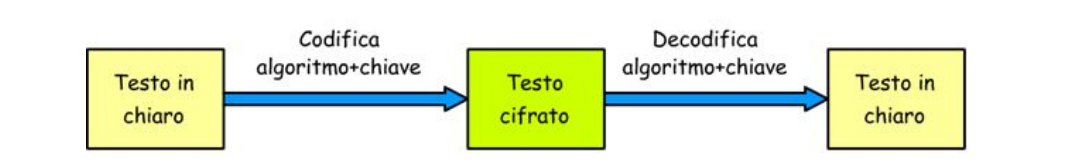
\includegraphics[width=\textwidth, keepaspectratio]{capitoli/crittografia/imgs/privata.png}
    \caption{Esempio del funzionamento della Crittografia Simmetrica.}
\end{figure}

La codifica e la decodifica sono eseguite dagli algoritmi crittografici assieme
ad una chiave che è la
stessa per entrambi i procedimenti. Tale chiave pertanto dovrà essere condivisa
tra le parti della
comunicazione. La segretezza, l'autenticazione e l'integrità dipendono dalla
segretezza della chiave.
Un sistema crittografico a chiave simmetrica molto conosciuto è il
\textbf{DES} ideato nel 1976 dalla IBM,
tuttora usato per cifrare files nei personal computer.
Questo sistema utilizza una chiave di 56 bit
(256 possibili chiavi).

\section{Crittografia a chiave Pubblica (asimmetrica)}

La crittografia asimmetrica, conosciuta anche come crittografia a coppia di chiavi,
crittografia a
chiave pubblica/privata o anche solo crittografia a chiave pubblica, è un tipo
di crittografia dove ad
ogni attore coinvolto nella comunicazione è associata una coppia di chiavi:

\begin{itemize}
    \item La chiave pubblica, che deve essere distribuita;
    \item La chiave privata, appunto personale e segreta;
\end{itemize}

Fra due interlocutori, non vi è dunque la necessità di scambiarsi le chiavi.
Se con una delle due
chiavi si cifra (codifica) un messaggio, allora quest'ultimo sarà decifrato solo
con l'altra.

\begin{figure}[H]
    \centering
    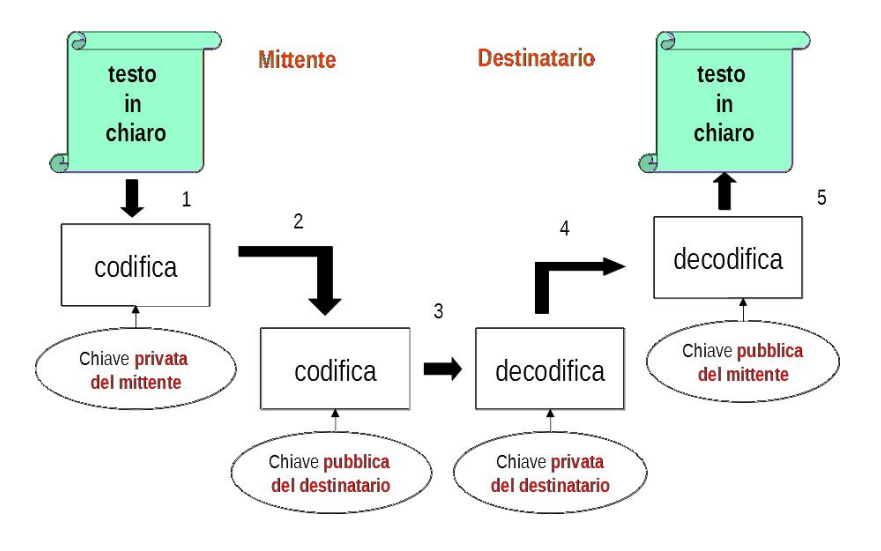
\includegraphics[width=\textwidth, keepaspectratio]{capitoli/crittografia/imgs/pubblica.png}
    \caption{Esempio del funzionamento della Crittografia Asimmetrica.}
\end{figure}

Gli attacchi a sistemi di crittografai sono detti attacchi
di \textbf{Crittoanalisi} e
come obbiettivo hanno quello di provare a dedurre la chiave che gli
permetterebbe di decriptare il testo.
I principali attacchi crittografici si basano sulle seguenti caratteristiche:

%%TODO: riscrivere a verso le varie descrizioni.
\begin{itemize}
    \item \textbf{CypherText only}: è noto solo il testo codificato;
    \item \textbf{Known plaintext}: il messaggio è cifrato ma il testo in chiaro è noto;
    \item \textbf{Chosen plaintext}: il testo in chiaro viene scelto in quale modo (per es. tutti 0, tutti 1, ecc);
    \item \textbf{Brute-force}: forza bruta, tentativi di attacco alla chiave finché non si trova quella giusta;
\end{itemize}

\paragraph{Crittografia Perfetta: } la crittografai si di dice Perfetta quando
nessun
testo codificato rilascia informazione alcuna né
sulla chiave usata per la codifica, né sul testo in chiaro,
il quale può essere recuperato se e solo se
la chiave è disponibile.
Si tratta di una situazione ideale, in quanto ogni tipo di crittoanalisi sarebbe
reso inutile e la
probabilità di ricavare informazioni supplementari da un testo codificato
sarebbe piuttosto nulla.
Purtroppo però, la crittografia in pratica non è quasi mai perfetta.

\section{Funzioni Hash}

Una funzione di hash è una funzione matematica che permette di ridurre una
qualunque stringa di
testo (indipendentemente dalla sua lunghezza) in una nuova stringa avente
precise caratteristiche
tra cui un numero di caratteri predefinito. A partire da un input X, in
altre parole, sarà possibile
generare un input Y che avrà delle caratteristiche ben definite.
A prescindere dal tipo di funzione di hashing tutte hanno dei punti in comune:

\begin{itemize}
    \item \textbf{Costanza}: a parità di input la stessa funzione di hash
          restituirà sempre la stessa stringa
          alfanumerica; ad ogni input, in altre parole, corrisponde sempre e
          inevitabilmente lo stesso
          output;
    \item \textbf{Irreversibilità}: mentre è sempre possibile riprodurre
          l'output conoscendo l'input originario
          col quale l'output è stato generato non è però possibile fare
          il percorso inverso, non si può
          quindi a partire da una stringa alfanumerica risalire al contenuto
          iniziale dell'input;
    \item \textbf{Determinismo}: indipendentemente da quanto sia lungo l'input,
          la funzione di hash restituirà
          sempre una stringa alfanumerica di un numero determinato di caratteri;
    \item \textbf{Effetto} valanga: non importa quanto l'input sia lungo e
          complesso, è sufficiente una
          variazione infinitesimale dell'input per generare un output
          completamente differente;
\end{itemize}

\section{Firma Digitale}

La firma digitale è una tecnologia con cui possono essere
effettivamente soddisfatti tutti i requisiti richiesti per dare validità
legale ad un documento elettronico firmato digitalmente;
garantisce i servizi di integrità, autenticazione e non ripudio.
Firmare non è esattamente codificare: firmare digitalmente un documento è spesso
utile perché evita di
codificare l'intero file in quanto ciò può richiedere un
tempo elevato. Verificare una firma, quindi, non significa
decodificare.

\begin{figure}[H]
    \centering
    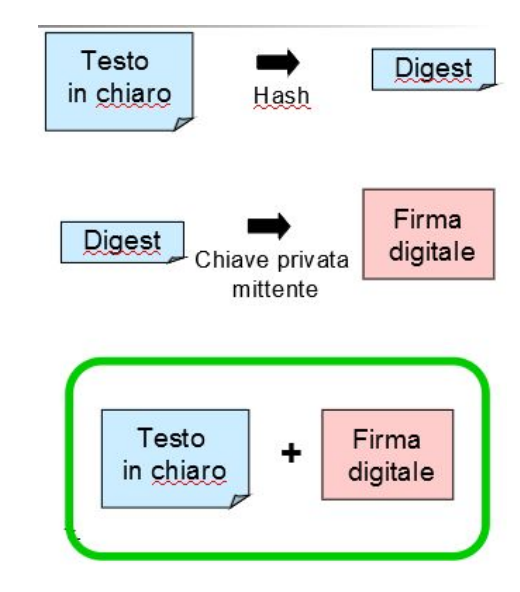
\includegraphics[width=\textwidth, keepaspectratio]{capitoli/crittografia/imgs/firmad.png}
\end{figure}

\subsection{Creazione della Firma}

La firma digitale viene realizzata tramite tecniche
crittografiche a
chiave pubblica insieme all'utilizzo di particolari
funzioni matematiche, chiamate funzioni hash
unidirezionali. Il processo di firma digitale passa
attraverso tre fasi:

\begin{enumerate}
    \item Generazione dell'impronta digitale.
    \item Generazione della firma.
    \item Apposizione della firma.
\end{enumerate}

Nella prima fase viene applicata al documento in
chiaro una funzione di hash appositamente
studiata che produce una stringa binaria di
lunghezza costante e piccola, normalmente 128 o 160
bit, chiamata “digest message”, ossia impronta
digitale.
Poiché la dimensione del digest message è fissa,
e molto più piccola di quella del messaggio
originale, la generazione della firma risulta
estremamente rapida. Utilizzare le funzioni hash
consente di evitare che per la generazione della
firma sia necessario applicare l'algoritmo di
cifratura all'intero testo che può essere molto lungo.
Mediante un software adatto si genera una coppia di
chiavi da utilizzare: una che verrà mantenuta
segreta per l'apposizione della firma; l'altra, destinata alla verifica, che
verrà resa pubblica. Quindi
la seconda fase, la generazione della firma, consiste semplicemente nella
cifratura con la propria
chiave privata dell'impronta digitale generata in precedenza.
Nell'ultima fase, la firma digitale generata precedentemente viene aggiunta in
una posizione
predefinita, normalmente alla fine del testo del documento.
E' da tenere presente che l'apposizione della firma digitale non garantisce la
confidenzialità del
testo, perché questo viene inviato in chiaro. Serve solo a garantirne integrità
e autenticità:

\begin{itemize}
    \item \textbf{Autenticità}: Il messaggio arriva proprio da chi dice di essere il mittente;
    \item \textbf{Integrità}: Il messaggio non ha subito modifiche o manomissioni;
\end{itemize}

\subsection{Verifica della Firma}

Il destinatario ottiene testo in chiaro con apposta la firma digitale.
Per comodità viene inviata anche la chiave pubblica del mittente. A
questo punto gli step sono:

\begin{enumerate}
    \item Separare il testo dalla firma;
    \item Decodificare la firma con la chiave pubblica del mittente;
    \item Calcolare il digest del testo tramite la funzione di hash;
    \item Verificare che i due digest coincidano. In caso positivo si ha
          la conferma del fatto che il documento è integro e non è stato
          sottoposto a modifiche.
\end{enumerate}